\documentclass[12pt]{article}
\usepackage[a4paper, width=150mm,top=25mm,bottom=25mm]{geometry}
\usepackage{amsmath}
\usepackage{amsfonts}
\usepackage{hyperref}
\usepackage[cache=false, outputdir=aux]{minted}
\usepackage{listings}
\usepackage{graphicx}
\graphicspath{attachments/}

\lstset{basicstyle=\ttfamily}

\begin{document}
\section{Simulation of Conservation laws}
\subsection{Trixi.jl}
\href{https://github.com/trixi-framework/Trixi.jl}{\lstinline[language=Python]|Trixi.jl|} is a numerical simulation framework for conservation laws written in 
\lstinline[language=Python]|Julia|.
\subsection{Features of {\ttfamily Trixi.jl}}

\lstinline[language=Python]|Trixi.jl| package can be used for conservation laws in $1$D, $2$D and $3$D dimensions with the following features:
\begin{itemize}
    \item Support cartesian and curvilinear meshes.
    \item Structured and Unstructured meshes.
    \item AMR and Shock capturing.
    \item High-order accuracy in space and time.
    \item Discontinuous Galerkin methods.
    \item CFL-based and error-based time step control.
    \item Periodic and weakly-enforced boundary conditions.
\end{itemize}
{\ttfamily Trixi.jl} has multiple governing equations such as {\ttfamily Compressible Euler, Compressible Navier-Stokes, Shallow water equations} etc.
The code written in this package also have support for {\ttfamily shared memory} parallelization via {\ttfamily multi-threading} and {\ttfamily multi-node} parallelization
via  {\ttfamily Message Passing Interface (MPI)}. It also provides visualization and post-processing support for the results.

It uses $Runge-Kutta$ methods for discretization in time with other high-orders for space discretization.

\subsection{{\ttfamily TrixiLW.jl}}
In {\ttfamily TrixiLW}, we have extended the {\ttfamily Trixi} package to use $Lax-Wendroff~flux\\reconstruction$ method for time discretization instead of $RK$ methods. 

\subsubsection{Features of {\ttfamily TrixiLW}}
{\ttfamily TrixiLW} can be used for conservation laws in $2$D with the following features:
\begin{itemize}
    \item Support for cartesian and curvilinear meshes.
    \item Structured and Unstructured meshes.
    \item High-order accuracy in space and time.
    \item Discontinuous Galerkin methods.
    \item CFL-based and error-based time step control.
    \item Periodic and non-periodic boundary conditions.
    \item AMR and Shock capturing
\end{itemize}
This package also supports {\ttfamily shared memory} parallelization via {\ttfamily multi-threading} and {\ttfamily multi-node} parallelization via {\ttfamily Message Passing
Interface (MPI)}. For visualization and post-processing, we use the tools of {\ttfamily Trixi} itself.

\subsubsection{{\ttfamily Multi-node} parallelization of {\ttfamily TrixiLW}}
{\ttfamily Multi-node} parallelization implies that we can use the computing units that not present on a single node on which the program is running. This can help us encounter
the issue of insufficient memory on a single node. We, now, can use memory of other nodes which are connected to each other via channel-based fabric such as {\ttfamily InfiniBand}
that facilitates high-speed communication between interconnected nodes. 

Although, using {\ttfamily multi-node} parallelization can also creates a communication overhead for the running program yet it is used since their is a nice trade-off between
the overhead created due to communication and other aspects such as memory, computing power, data storage etc. 

Message Passing Interface (MPI) is an open source implementation that laid down the rules for communication routines between processes. It is developed and maintained by MPI Forum.
There are many open source libraries that are based on MPI and prvoide language specific routines. These includes {\ttfamily OpenMPI, MPICH} etc.

\subsubsection{Idea of parallelization}
{\ttfamily TrixiLW.jl} is based on Lax-Wendroff Flux reconstruction (LWFR) method. In this method, as explained in the previous section, we need $u$ (solution values), $U$ (time average
solution) and $F$ (time average flux) values to be communicated to other required ranks.

\begin{figure}[!ht]
    \centering
    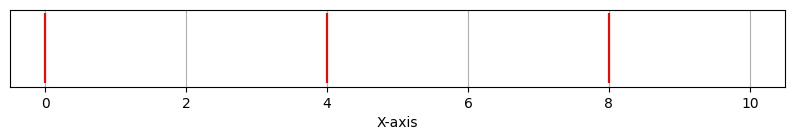
\includegraphics[width=0.9\linewidth]{../attachments/1Dmesh.png}
    \caption{interfaces and mpi\_interfaces}
    \label{1}
\end{figure}
In figure(\ref{1}), the red lines are {\ttfamily mpi\_interfaces} which are not owned by the current rank and grey lines are {\ttfamily interfaces} which are owned by the current rank.
The values need to be communicated only at the {\ttfamily mpi\_interfaces}
and not at the normal {\ttfamily interfaces}. We have used non-blocking communication routines for communication between ranks. These routines include: {\ttfamily MPI\_Isend} and
{\ttfamily MPI\_Irecv}.

\subsubsection{Data Structures}
At each interface, as we have seen, three variables needs to be stored $u$, $U$ and $F$, following is the {\ttfamily MPIInterfaceContainer} data structure that will be used to store data.
\\ \vspace{21pt}
\begin{listing}[!ht]
\centering
\begin{minted}[linenos]{Julia}
# Container data structure (structure-of-arrays style) 
# for DG MPI interfaces
mutable struct MPIInterfaceContainerLW2D{uEltype <: Real}
                                         <:AbstractContainer
    u::Array{uEltype, 4}     # [leftright, variables, i, interfaces]
    U::Array{uEltype, 4}
    F::Array{uEltype, 4}
    local_neighbor_ids::Vector{Int} # [interfaces]
    orientations::Vector{Int}       # [interfaces]
    remote_sides::Vector{Int}       # [interfaces]
    # internal `resize!`able storage
    _u::Vector{uEltype}
    _U::Vector{uEltype}
    _F::Vector{uEltype}
end
\end{minted}
\caption{Struct for mpi\_interfaces}
\end{listing}
% \hrule
The {\ttfamily struct} below has some extra fields for such as $\_u$, $\_U$ and $\_F$, these field are needed for internal storage as in {\ttfamily Julia} only 1D arrays can be resized.
Therefore, memory will be allocated for these 1D arrays and data will be stored in them. Later, that allocated memory will again be used using {\ttfamily unsafe\_wrap} method of {\ttfamily Julia}
without making another copy of data hence avoiding unnecessary memory allocation.

Other field as {\ttfamily local\_neighbor\_ids} will store {\ttfamily ranks} of neighboring interfaces, {\ttfamily orientations} will store the orientation of the interface (either x or y direction)
and {\ttfamily remote\_sides} will contain the information whether {\ttfamily mpi\_interfaces} are in positive direction or negative direction of the axis.

There will be another function called {\ttfamily prolong2mpiinterfaces!} which will be responsible for prolonging the element data to {\ttfamily mpi\_interfaces} and filling up the above mentioned
container.
\end{document}